\chapter{Operatori per l'elaborazione digitale delle immagini}\lb{OEDI}

%======================================================================================
\section{Cambiamento di risoluzione}

Le immagini analogiche generate da un sistema ottico per poter essere memorizzate ed
elaborate vengono campionate nelle coordinate spaziali e quantizzate nell'intensit\a.
La suddivisione dell'immagine in $M$ righe e $N$ colonne individua un numero finito
$M \cdot N$ di elementi d'immagine ({\it pixel}); $M$ ed $N$ specificano quindi la risoluzione
dell'immagine.
In alcuni casi un'alta definizione pu\o risultare non indispensabile e anzi costituire
un limite all'efficienza dell'algoritmo in quanto si ha un elevata quantit\a di dati da
analizzare.
Inoltre vi sono applicazioni in cui si sfrutta la possibilit\a di analizzare l'immagine a
diverse scale di definizione per poter individuare alcune strutture dell'imma-gine che
risultano invarianti al variare della risoluzione.
In particolare con l'adozione di opportune strutture dati come la piramide di immagini 
(\cite{Zamperoni}, \cite{Meer}).

%-------------------------------------------------------------------------------------
\subsection{Riduzione della risoluzione}

La trasformazione che porta alla riduzione della risoluzione mappa necessariamente diversi
punti dell'immagine ad alta risoluzione in un punto di quella a risoluzione inferiore.
Il caso pi\u semplice \e dato dal campionamento in cui si considerano, ad esempio, i punti
dell'immagine ad indici dispari:

\vs(5)

sia $f\,(\,x\,,\,y\,)$ l'immagine di partenza di dimensioni $(\,R,C\,)$, con $R$ e $C$
pari, allora  
\be
h\,(\,x\,,\,y\,)\,=\,f\,(\,2\,x\,-\,1\,,\,2\,y\,-\,1\,)
\lb{campion}
\ee

con le due dimensione ridotta di un fattore $2$. 

\vs (5)

A causa della riduzione della risoluzione si pu\o avere una perdita nella definizione di 
alcuni dettagli dell'immagine; tale perdita di informazione che pu\o essere limitata
con un'opportuna scelta del nucleo della trasformazione stessa, per esempio considerando
la media del valore dei pixel nell'intorno del punto considerato\footnotemark:
\beqa
h\,(\,x\,,\,y\,) & = & \frac{1}{4}\,[\,f\,(\,2\,x\,-\,1\,,\,2\,y\,-\,1\,)\,+\, 
                                     f\,(\,2\,x\,-\,1\,,\,2\,y\,)\,+ \nonumber\\
                 &   &              +\,f\,(\,2\,x\,,\,2\,y\,-\,1\,)\,+\,
                                     f\,(\,2\,x\,,\,2\,y\,-\,1\,)\,]
\lb{media}
\eeqa
\footnotetext{La costruzione della piramide di immagini pu\o essere visto come un processo
di decimazione, per cui il nucleo che rende minima la perdita d'informazione dovuta al
campionamento, ovvero che permette la ricostruzione dell'immagine originale, \e il filtro
passa-basso ideale.}

Per un maggior approfondimento sulla scelta del nucleo si pu\o far riferimento a quanto
riportato in \cite{Meer}.

%======================================================================================
\section{Trasformazioni dello spazio dei colori}

Generalmente le immagini a colori sono rappresentate per mezzo del modello $RGB$, dove ad ogni
pixel \e associato un vettore tridimensionale le cui componenti sono proprio i valori
di rosso $R$, verde $G$ e blu $B$ in cui \e possibile scomporre il colore percepito del pixel.

Una rappresentazione di questo tipo \e per\o legata alle caratteristiche del sensore (CCD) che
ha fornito l'immagine per cui spesso si ricorre ad altri spazi in cui rappresentare le 
propriet\a intrinseche del colore meno sensibili alle 
caratteristiche del sensore stesso.

Esiste una vasta gamma di possibili modelli, trasformazioni, metriche che possono essere
utilizzate per evidenziare le propriet\a utili alle diverse applicazioni \cite{Wyszecki}; nel nostro
caso si sono considerate la trasformazione che permette di ottenere le componenti $HSI$
del colore e la {\it trasformazione di Karhunen-Lo\`eve}.

%-------------------------------------------------------------------------------------
\subsection{Lo spazio HSI}

La trasformazione che mappa lo spazio $RGB$ nello spazio $HSI$ (o $HSV$) \e non lineare con
alcune singolarit\a:
\bi

\im (\,{\it Hue}\,) {\it Tonalit\a}: caratterizza il colore dominante nel punto {\bf x} 
    del-l'immagine.
    Una possibile rappresentazione dello spazio della coordinata pu\o essere quello
    di figura. 

    \begin{figure}[h]
    \centerline{
     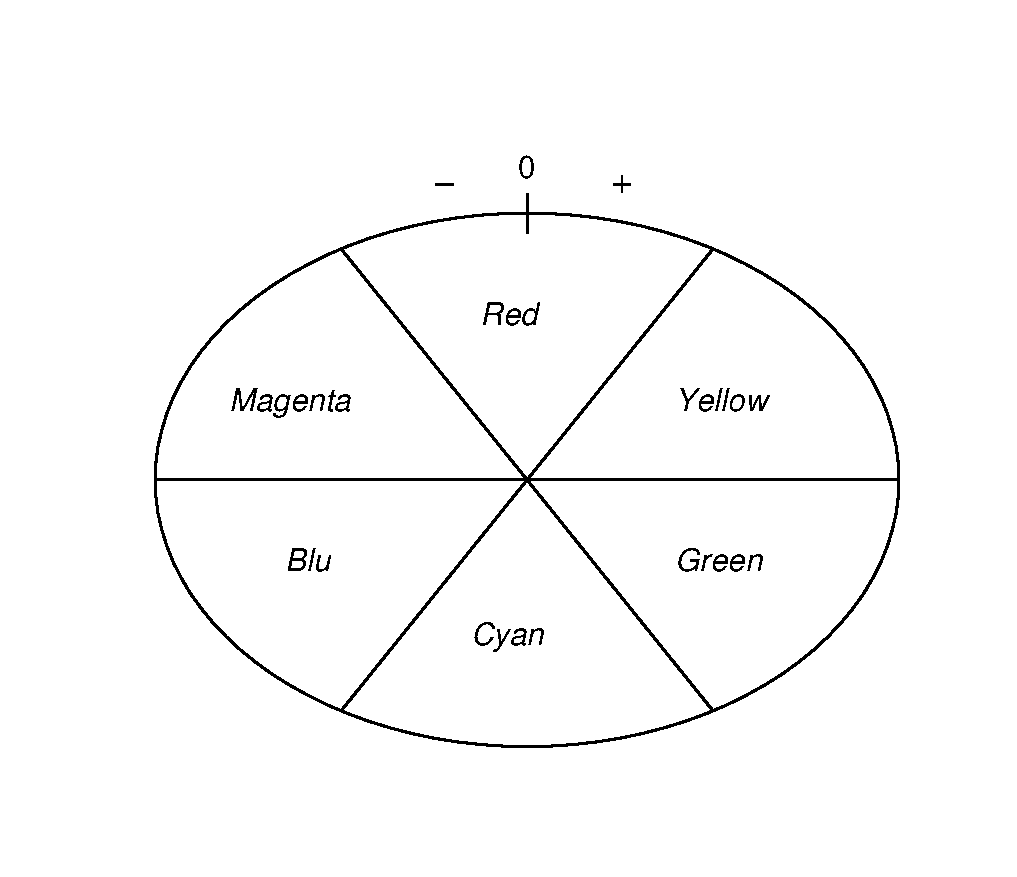
\psfig{file="./images/hsi.eps",width=5.8cm,height=5cm,bbllx=80pt,bblly=260pt,bburx=560pt,bbury=570pt,clip=}}
    \caption{Rappresentazione dello spazio della coordinata ${\it Hue}$}
    \end{figure}


    E' pu\o essere definita formalmente 
    \be
    H\,=\,\arctan\,(\,\sqrt{3}\,(\,G\,-\,B\,),2\,R\,-\,G\,-\,B\,)
    \ee
    
    che vale $0$ in presenza della sola componente monocromatica $R$.

\im (\,{\it Intensity}\,) {\it Luminosit\a}:
    \be
    I\,=\,\frac{R\,+\,G\,+\,+\,B}{3}
    \ee

    vale $0$ nel caso del colore nero ed \e massima per il bianco.

\im (\,{\it Saturation}\,) {\it Saturazione} o {\it Purezza}: misura il rapporto fra
    la componente monocromatica dominante e quella bianca necessarie ad ottenere
    il colore del punto.
    \be
    S\,=\,1\,-\,3\,\frac{\min\,\{\,R,G,B\,\}}{I}
    \ee    
    $S\,=\,1$ denota un colore puro, mentre vale $S\,=\,0$ se bianco ($R\,=\,G\,=\,B\,=\,1$).

\ei

Alternativamente alla componente $I$ si pu\o trovare la componente $V$ definita

\bi

\im {\it Value}:
    \be
    V\,=\,\max\,\{R,G,B\}
    \ee
 
\ei

%-------------------------------------------------------------------------------------
\subsection{Trasformata di Karhunen-Lo\`eve o di Hotelling}

La {\it trasformata di Karhunen-Lo\`eve o di Hotelling}, con le sue varianti, \e la trasformazione
che permette di ottenere i migliori risultati nei problemi di segmentazione  \cite{Lee},
\cite{Schmid} e di analisi della tessitura ({\it texture}) \cite{Wouver} rispetto ai diversi 
modelli di colore.
L'effetto della {\it trasformata di Hotelling} sui vettori di un dato spazio \e quello di
proiettarli in un nuovo spazio con le stesse dimensioni dove per\o ora le componenti 
risultano statisticamente scorrelate.

\vs(10)

Di seguito consideriamo la definizione della trasformazione applicata al caso di 
immagini a colori definite nello spazio $RGB$:

\vs(5)

dati i pixels ${\bf x}$ dell'immagine $I$, si considerano il vettore media e
la matrice di covarianza

\be
{\bf m}\,=\,E\,[\,{\bf x}]
\ee
\be
{\bf k}\,=\,E\,[\,(\,{\bf x}\,-\,{\bf m}\,)\,(\,{\bf x}\,-\,{\bf m}\,)^T\,]
\ee

In pratica si sostituiscono con le rispettive media e covarianza campionaria.

Si procede calcolando gli autovalori $\lambda_i$ e gli autovettori ${\bf e}_i$ della
matrice di covarianza ${\bf k}$; quindi si costruisce la matrice ${\bf A}$ le cui righe
sono gli autovettori ordinati secondo autovalori decrescenti.
La {\it trasformazione di Hotelling} \e ottenuta semplicemente
\be
{\bf y}\,=\,{\bf A}\,(\,{\bf x}\,-\,{\bf m}\,)
\lb{kltrasf}
\ee

Per verificare che le componenti degli ${\bf y}$ sono incorrelate si consideri la 
matrice di covarianza che in questo caso \e anche di correlazione in quanto sono
vettori a media nulla, infatti
\be
{\bf m_y}\,=\,E\,[\,{\bf y}]\,=\,{\bf A}\,(\,E\,[\,{\bf x}\,]\,-\,{\bf m}\,)\,=\,{\bf 0}
\lb{vmediay}
\ee
\be
{\bf k_y}\,=\,E\,[\,(\,{\bf y}\,-\,{\bf m_y}\,)\,(\,{\bf y}\,-\,{\bf m_y}\,)^T\,]
\,=\,{\bf A}\,{\bf k}\,{\bf A}^T
\lb{mcovy}
\ee

Tenendo presente che la matrice di covarianza ${\bf k}$ \e simmetrica, allora esiste
una matrice ortogonale, le cui righe formano una base ortonormale dello spazio $RGB$,
che la diagonalizza. 
La matrice ortogonale \e proprio ${\bf A}$, le cui righe sono gli autovettori di ${\bf k}$,
per cui la matrice diagonale risultante \e ${\bf k_y}$; ci\o significa che
le componenti di ${\bf y}$ sono statisticamente scorrelate e con varianza data
dagli autovalori, elementi della diagonale della matrice di covarianza.

\vs(5)

Dallo sviluppo della {\it trasformata di Hotelling} si osserva che essa permette
di scomporre l'immagine secondo le sue componenti principali valutate lungo
le direzioni a massima varianza.
Questo permette sia di limitare le trasformazioni successive alle componenti di
maggior rilievo, con un risparmio computazionale, sia di migliorare la qualit\a
delle trasformazioni successive in quanto \e possibile scartare le componenti
caratterizzate da una minor varianza (autovalori minori) che sono pi\u sensibili
al rumore (minore $SNR$).

A partire dai vettori trasformati ${\bf y}$ \e possibile riottenere i vettori
dello spazio originario ${\bf x}$ applicando la trasformazione inversa 

\be
{\bf x}\,=\,{\bf A}^{-1}\,{\bf y}\,+\,{\bf m}
\ee

con ${\bf A}^{-1}\,=\,{\bf A}^T$ per l'ortogonalit\a.

Se ora si considerano solo i primi $n$ autovettori e le prime $n$ componenti di ${\bf y}$,
si ricava

\be
\hat{\bf x}\,=\,{\bf A}^T_n\,{\bf y}_n\,+\,{\bf m}
\lb{klappr}
\ee

che rappresenta una approssimazione di ${\bf x}$.

Rilevante \e il fatto che \e possibile stabilire l'errore di approssimazione, ovvero 
la sua potenza statistica, in modo immediato data l'ortogonalit\a delle componenti.
Se $N$ \e il numero totale degli autovalori la potenza dell'errore di stima

\be
P_e\,=\,\sum_{i=n+1}^{N}\,\lambda_i
\ee

Tenendo quindi presente che gli autovalori sono ordinati in modo decrescente tale errore
risulta minimo fissato $n$.

\boss
La trasformata di Karhunen-Lo\`eve dipende, attraverso gli
autovettori della matrice di covarianza, dalle caratteristiche dell'immagine
in esame; si \e verificato per\o \cite{Ohta} che tali autovettori rimangono
pressoch\e invariati per un vasto insieme di immagini di sogetti reali.
\eoss

Quindi la trasformata si pu\o semplificare nella forma

\be
\pmatrix{K_1 \cr
         K_2 \cr
         K_3 \cr} 
\,=\,
\smatrix{3}{ \frac{1}{3} & \frac{1}{3} &  \frac{1}{3} \cr
             \frac{1}{2} &           0 & -\frac{1}{2} \cr
            -\frac{1}{2} &           1 & -\frac{1}{2} \cr}
\,
\pmatrix{R \cr
         G \cr
         B}
\ee  

Si osservi che la prima componente \e definita come l'{\it Intensit\a} in $HSI$.

%======================================================================================
\section{Operatori Morfologici}

Sono una classe importante di operatori locali che operano sulla forma degli elementi
che compaiono nell'immagine.
Gli operatori morfologici vengono utilizzati per eliminare piccoli oggetti, fessure,
buchi, regolarizzare i bordi e per individuare i bordi ({\it edge-detection}); oppure
per estrarre degli oggetti noti da un'immagine ({\it shape analysis \& pattern classification}).
 
La teoria alla base di tali trasformazioni, da cui mutuano il nome, \e la {\it matematica
morfologica} che si sviluppa a partire dalla teoria degli insiemi che assumono, in
tale contesto, un significato particolare.
In questo paragrafo si propone una breve introduzione ai due operatori base, {\it dilatazione}
({\it dilation}) ed {\it erosione} ({\it erosion}), e le due trasformazioni fondamentali,
ottenute dalle precedenti, {\it apertura} ({\it opening}) e {\it chiusura} ({\it closing}).
Per un maggior approfondimento si rimanda ai riferimenti \cite{Haralick87},\cite{Haralick92}
dello stesso autore in cui si possono trovare, oltre alle dimostrazioni, maggiori
argomentazioni sull'importanza di tali operatori e diverse indicazioni sulle possibili
applicazioni. 

\vs(5)

Di seguito si considerano le definizioni dei diversi operatori e le loro principali
propriet\a in particolare in relazione alla loro implementazione.

%-------------------------------------------------------------------------------------
\subsection{Dilatazione ed Erosione}

\bdf

Siano $A$ e $K$ due sottoinsiemi di $\M(E)^N$, si definisce {\bf dilatazione} di $A$ data $K$
\be
A\,\oplus\,K\,=\,\{\,c\,\in\,\M(E)^N\,:\,c\,=\,a\,+\,k,\,a\,\in\,A,\,k\,\in\,K\,\}
\ee

si definisce {\bf erosione} di $A$ dato $K$
\be
A\,\ominus\,K\,=\,\{\,c\,\in\,\M(E)^N\,:\,c\,+\,k\,\in\,A,\,\forall\,k\,\in\,K\,\}
\ee

\edf

\boss
In generale i termini $A$ e $K$ sono due generici sottoinsiemi dello spazio $\M(E)^N$,
in realt\a il primo operando \e l'immagine che si sta elaborando mentre il secondo
costituisce il nucleo o elemento strutturale ({\it structuring element}) della 
trasformazione rappresentante un parametro di forma di un elemento dell'immagine.
\eoss

Per implementare in modo pi\u efficiente i due operatori \e opportuno esprimerli come 
combinazioni dell'immagine traslata

\bdf
Dati $A\,\subseteq\,\M(E)^N$, $x\,\in\,\M(E)^N$, si definisce traslazione di $A$ dato $x$
\be
A_x\,=\,\{\,c\,\in\,\M(E)^N\,:\,c\,=\,a\,+\,x,\,a\,\in\,A\,\}
\ee
\edf

\bpr
\be
A\,\oplus\,K\,=\,\bigcup_{k \in K}\,A_k
\lb{tr_dil}
\ee

\be
A\,\ominus\,K\,=\,\bigcap_{k \in K}\,A_{-k}
\ee
\epr

\bpr
 Gli operatori di {\it dilatazione} ed {\it erosione} soddisfano le seguenti propriet\a:

\bi

\im {\bf Commutativa}. Vale solo per l'operatore di {\it dilatazione}. 
    \be
    A\,\oplus\,K\,=\,K\,\oplus\,A 
    \lb{com_dil}
    \ee

\im {\bf Associativa}. Sia $K\,=\,K_1\,\oplus\,K_2$
    \beqa
    \lb{assde}
    A\,\oplus\,K & = & A\,\oplus\,(\,K_1\,\oplus\,K_2\,)\,=\,(\,A\,\oplus\,K_1\,)\,\oplus\,K_2 \\
    A\,\ominus\,K & = & A\,\ominus\,(\,K_1\,\ominus\,K_2\,)\,=\,(\,A\,\ominus\,K_1\,)\,\ominus\,K_2 \nonumber
    \;\;\;\;\;\;\;\;
    \eeqa
    
\im {\bf Distributiva}.

    Fra le possibili combinazioni si considerano in particolare
    \beqa
	\lb{dist}    
    A\,\oplus\,(\,B\,\cup\,C\,) & = & (\,A\,\oplus\,C)\,\cup\,(\,A\,\oplus\,C\,) \\
    %-------------------------------------------------------------------------------   
    A\,\ominus\,(\,B\,\cup\,C\,) & = & (\,A\,\ominus\,C)\,\cap\,(\,A\,\ominus\,C\,) \nonumber
    \eeqa

\ei    
\epr

\boss
Dalle (\ref{assde}) e (\ref{dist}) si possono ricavare due
soluzioni per scomporre il nucleo della tarsformazione ({\it structuring element});
la differenza \e che nelle (\r{assde}) si ottiene una cascata di operazioni elementari
mentre nelle (\r{dist}) tali operazioni sono eseguibili in parallelo.
\eoss

Esiste anche un teorema di dualit\a che lega i due operatori.

\bth
{\bf Dualit\a.}

$$
(\,A\,\ominus\,B\,)^c\,=\,A^c\,\oplus\,\check{B} 
$$

dove $\check{B}\,=\,\{\,x\,:\,\exists\,b\,\in\,B\,:\,x\,=\,-\,b\,\}$

e $(\,^c\,)$ \e l'usuale operazione di complemento rispetto l'insieme $\M(E)^N$.
\eth

Il teorema mette in luce il fatto che le due operazioni non sono l'una l'inversa
dell'altra nel senso usuale del termine, ma si possono considerare complementari.
Nel senso che se si considera la dilatazione di un insieme $A\,\subseteq\,\M(E)^N$,
\e possibile in modo duale ottenere lo stesso risultato con un'operazione di
erosione sull'insieme complementare.
In particolare nel caso in cui il nucleo ({\it structuring element}) sia simmetrico,
per cui $\check{K}\,=\,K$, si ha che l'erosione di $A$ dato $K$ \e perfettamente
complementare alla dilatazione di $A^c$ dato $K$.

\vs(5)

Prima di introdurre i due operatori fondamentali della matematica morfologica
\e opportuno considerare il seguente risultato

\bpr

$$
A\,\oplus\,(\,B\,\ominus\,C\,)\,\subseteq\,(\,A\,\oplus\,B\,)\,\ominus\,C
$$

\epr

che evidenzia l'importanza dell'ordine di applicazione dei due operatori {\it dilatazione}
ed {\it erosione}.

%-------------------------------------------------------------------------------------
\subsection{Apertura e Chiusura}

In pratica le due operazioni considerate nella sezione precedente non sono quasi mai
utilizzate singolarmente ma combinate per realizzare le due trasformazioni fondamentali 
di {\it apertura} ({\it opening}) e {\it chiusura} ({\it closing}).

\bdf

Si definisce {\bf apertura} di $A$ dato $K$

\be
A\,\circ\,K\,=\,(\,A\,\ominus\,K\,)\,\oplus\,K.
\ee

Se $A\,\circ\,K\,=\,A$ si dice che $A$ \e {\bf aperto} rispetto $K$.

Si definisce {\bf chiusura} di $A$ dato $K$

\be
A\,\bullet\,K\,=\,(\,A\,\oplus\,K\,)\,\ominus\,K.
\ee

Se $A\,\bullet\,K\,=\,A$ si dice che $A$ \e chiuso rispetto $K$.

\edf

Una propriet\a importante dei due operatori \e l'idempotenza.

\bth
{\bf Idempotenza.}
\beqa
(\,A\,\circ\,K\,)\,\circ\,K & = & A\,\circ\,K \\
(\,A\,\bullet\,K\,)\,\bullet\,K & = & A\,\bullet\,K \nonumber
\eeqa
\eth

Vale anche una relazione di dualit\a da intendersi come per i due operatori precedenti. 

\bth
{\bf Dualit\a.}
\be
(\,A\,\bullet\,K\,)^c\,=\,A^c\,\circ\,\check{K}
\ee
\eth

Un'interpretazione geometrica dell'azione dei due operatori \e data dal seguente risultato.

\bpr

\be
A\,\circ\,K\,=\{\,x\,\in\,A\,:\,\exists\,y\,:\,x\,\in\,K_y\,\subseteq\,A\,\}
\,=\,\bigcup_{\{y\,:\,K_y\subseteq\,A\}}\,K_y
\ee

\epr

Esprime l'operazione di {\it apertura} come l'unione di tutte le possibili traslazioni
di $K$ che sono contenute in $A$.

Sfruttando la dualit\a si ha invece che l'operazione di {\it chiusura} \e otenuta
come il complemento dell'unione di tutte le traslazioni di $\check{K}$ contenute
in $A^c$.

%-------------------------------------------------------------------------------------
\subsection{Operatori morfologici per immagini binarie}

Nel caso particolare di immagini binarie gli operatori morfologici si riducono ad
espressioni logiche a cui \e possibile applicare le regole dell'algebra di Boole.

Si consideri l'operazione di {\it dilatazione} espressa nella forma (\r{tr_dil}) con
$A$, il sottoinsieme che definisce gli oggetti presenti e i cui pixels assumono valore $1$
({\it foreground}), e $K$ che assume valori in $\{0,1\}$; allora

$$
A\,\oplus\,K\,=\,\bigcup_{k\,\in\,K}\,A_k\,=\,\bigcup_{a\,\in\,A}\,K_a
$$

dove nell'ultimo passagio si \e sfruttata la commutativit\a dell'operatore (\r{com_dil}).

La {\it dilatazione} \e quindi ottenuta centrando la maschera $K$ su tutti i pixel
di $A$ e commutando ad $1$ tutti i pixels vicini che assumono eventualmente il
valore $0$ appartenenti a $A^c$ ({\it background}).

Tale operazione pu\o essere realizzata considerando gli operatori logici $and\,\wedge$ e
$or\,\vee$ tra l'immagine $I\,\supseteq\,A$ e la maschera $K$. Nell'ipotesi verosimile
che quest'ultima sia definita da una finestra-matrice simmetrica di dimensioni 
$(\,2\,n\,+\,1,2\,n\,+\,1\,)$ si ricava

\be
\hat{I}\,(\,r,c\,)\,=\,\bigvee_{i\,=\,-n}^{n}\,\bigvee_{j\,=\,-n}^{n}
\,K\,(\,i,j\,)\,\wedge\,I\,(\,r\,-\,i,c\,-\,j\,)
\ee

A questo punto \e possibile ottenere un'espressione anche per l'{\it erosione} sfruttando
la dualit\a e tenedo conto che $K$ \e simmetrica per cui $\check{K}\,=\,K$ e che
il complemento \e dato dalla negazione

\be
\hat{I}\,(\,r,c\,)\,=\,\overline{\bigvee_{i\,=\,-n}^{n}\,\bigvee_{j\,=\,-n}^{n}
\,K\,(\,i,j\,)\,\wedge\,\overline{I\,(\,r\,-\,i,c\,-\,j\,)}}
\ee

Definiti questi due operatori \e possibile ottenere per composizione anche quelli
pi\u complessi.

%-------------------------------------------------------------------------------------
\subsection{Operatori morfologici per immagini in scala di grigio}

Anche in questo caso le espressioni viste in generale assumono una forma pi\u
semplice una volta che si \e stabilito di lavorare con immagini a toni di grigio.
Lo spazio considerato \e $\M(E)^N\,=\,\M(E)^3$ dove le prime due componenti di ciascun
vettore sono le coordinate del punto dell'immagine mentre la terza rappresenta
il valore dell'intensit\a dell'immagine nel punto.

Per le immagini in scala di grigio le due operazioni che permettono di definire
la {\it dilatazione} e l'{\it erosione} sono quelle di {\it massimo} e {\it minmo}
rispettivamente

\bpr

Siano $F,K\,\subseteq\,\M(E)^2$, $f\,:\,F\,\rightarrow\,\M(E)$ e $k\,:\,K\,\rightarrow\,\M(E)$

\beqa
(\,f\,\oplus\,k\,)(\,x\,) & = & \max_{\matrix{\scriptstyle{\{\,y\,\in\,K,}\cr\scriptstyle{x\,-\,y\,\in\,F\,\}}}}\,
\{\,f\,(\,x\,-\,y\,)\,+\,k\,(\,y\,)\,\} \\
(\,f\,\ominus\,k\,)(\,x\,) & = & \min_{\{\,y\,\in\,K\,\}}\,
\{\,f\,(\,x\,+\,y\,)\,-\,k\,(\,y\,)\,\} \nonumber
\eeqa

\epr
 
Da cui \e possibile ottenere tutti gli altri operatori applicando le definizioni
date precedentemente.

%======================================================================================
\section{Rank-order filters - Mediana}

Rappresentano una classe di operatori locali non lineari che dipendono dal-l'ordinamento
dei valori definiti in una finestra $K\,(\,n,n\,)$, con $n$ dispari, centrata su ogni pixel
dell'immagine $I\,(\,R,C\,)$.

A partire da ${\bf v}_K$, vettore ordinato con valori crescenti, si possono ottenere
$n^2$ possibili risultati associati ai ${\bf v}_K\,(i)$, con $i$ ordine del filtro,
assegnabili al pixel centrale, oggetto dell'elaborazione. 

Se $i=1$ si ha il $min$, con $i=n^2$ il $max$ e con $i=(n^2+1)/2$ la
$mediana$ del vettore, che presenta alcune propriet\a interessanti \cite{Zamperoni}
e \cite{Haralick92}.

\boss
Nella costruzione del vettore ${\bf v}_K$ si \e considerato anche il pixel centrale
della finestra mentre in letteratura si possono trovare anche altre formulazioni che lo escludono.
In questi casi bisogna fare attenzione che se $n$ \e dispari allora $n^2-1$, il numero
di elementi del nuovo vettore ${\bf v}_K^\prime$, \e pari e si hanno due possibili valori
di mediana per $i=(n^2-1)/2$ e $i=(n^2-1)/2+1$. 
\eoss

I {\it rank-order filters} in generale e l'{\it operatore mediana} in particolare, con 
le loro varianti, vengono utilizzati sia per ridurre il rumore presente nell'immagi-ne
({\it image enhancement}) sia come componente per l'estrazione di particolari 
caratteristiche ({\it features}) dell'immagine, quali pattern lineari.
 
%======================================================================================
\section{Misura dell'anisotropia locale}

Bisogna considerare che all'interno di immagini, soprattutto quelle naturali, vi sono
particolari con caratteristiche spesso molto diverse tra di loro.

La possibilit\a di adattare l'operatore alle propriet\a locali dell'immagine permette di
soddisfare delle condizioni che potrebbero risultare altrimenti incompatibili, come 
ridurre il rumore e contemporaneamente conservare o migliorare la definizione dei bordi
({\it edge sharpness}) e dei dettagli.

Bisogna a questo punto definire uno o pi\u parametri che caratterizzino il comportamento del
filtro nei diversi punti dell'immagine.
Ci\o viene realizzato attraverso una {\it misura di anisotropia} che rivela la propriet\a di interesse
come, ad esempio, i punti appartenenti ai bordi (si veda il caso della {\it diffusione anisotropa}
ottenuta variando la forma del filtro gaussiano,
che \e per sua natura isotropo, in funzione del gradiente dell'immagine \cite{Perona}, \cite{Fischl}).  

\vs(5)

Una semplice definizione di anisotropia \e data dalla funzione $\alpha(p)$, misura di anisotropia nel
punto $p$, che stabilisce se il punto $p$ appartiene ad una regione uniforme, $\alpha(p)=0$,
o a una retta (pattern lineare filiforme e ben definito rispetto allo sfondo), $\alpha(p)=1$.

\bdf
Definita una finestra $K(\,n,n\,)$, con $n$ dispari, centrata sul pixel $p$, \e possibile
individuare $T=2\,(n-1)$ {\bf digital straight line segments} passanti per il punto $p$ e che
connettono due punti del bordo della finestra $K$ come in figura (\r{digseg}).
%(L'algoritmo che costruisce tali segmenti \e riportato in Appendice).
Si consideri $M_t$, con $t=1,\dots,T$, la media dell'intensit\a $I(x,y)$ lungo il segmento 
$t-esimo$ moltiplicato per $n$
\be
M_t\,=\,\sum_{i=-z}^{z}\,I\,(\,x+dx(t,i),y+dy(t,i)\,), \qquad z=(n-1)/2
\ee

dove $dx(t,i)$ e $dy(t,i)$ contengono gli spostamenti relativi tra il punto $p(x,y)$ su cui
\e centrata la finestra e i punti appartenenti alla retta $t-esima$.

Si definiscono ora $m_K(p)$ e $M_K(p)$
\bary(2)
m_K(p)\,=\,{\displaystyle{\min_{\matrix \scriptstyle t=1,\dots,T}}}\,\{\,M_t\,\} \quad
 & M_K(p)\,=\,{\displaystyle{\max_{\matrix \scriptstyle t=1,\dots,T}}}\,\{\,M_t\,\} 
\eary

A questo punto \e possibile definire la misura $\alpha(p)$ dell'anisotropia locale
\[
\alpha(p)=\cases{0 & se $M_K(p)=0$ \cr
                 {\displaystyle\frac{M_K(p)-m_K(p)}{M_K(p)+m_K(p)}} & altrimenti. \cr}
\lb{lam}
\]
 
\edf

\begin{figure}[tbp]
 \centerline{
  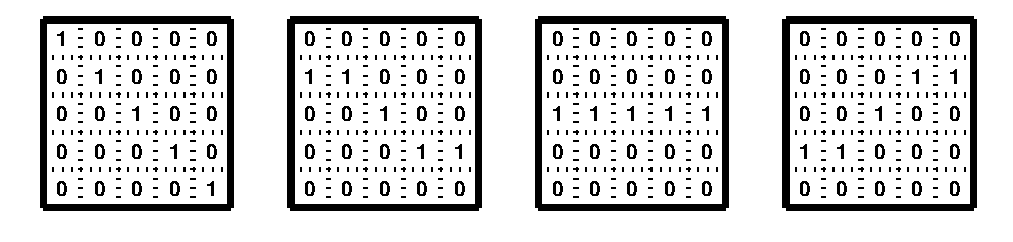
\psfig{file="./images/digseg1.eps",height=3cm,bbllx=80pt,bblly=350pt,bburx=550pt,bbury=450pt,clip=}}
 \centerline{
  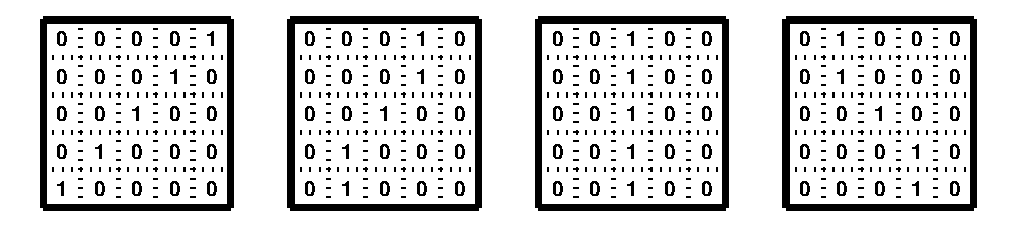
\psfig{file="./images/digseg2.eps",height=3cm,bbllx=80pt,bblly=350pt,bburx=550pt,bbury=450pt,clip=}}
 \caption[Digital straight line segments]
  {Gli $2\,(n-1)=8$ possibili {\it digital straight line segments} distinti passanti per il
   pixel $p$, al centro della maschera $K(n,n)$, nel caso di $n=5$}
 \lb{digseg}
\end{figure}

\finepar
 





